% SOURCE: submissions/d2-neurocomputing/zenodo-deposit/results/merging/RG_gain_law_MERGED_REFIX20260730.json :: bundles.*.{gain_median_absdrop_per_dose,frac_drop_negative} (22 protocol cells; cut=8; ordering_test.n_bundles=22) + submissions/d2-neurocomputing/zenodo-deposit/results/merging/RG_gain_holdout_20260716.json :: orderings CI fields (plotted bounds)
% !TEX encoding = UTF-8 Unicode
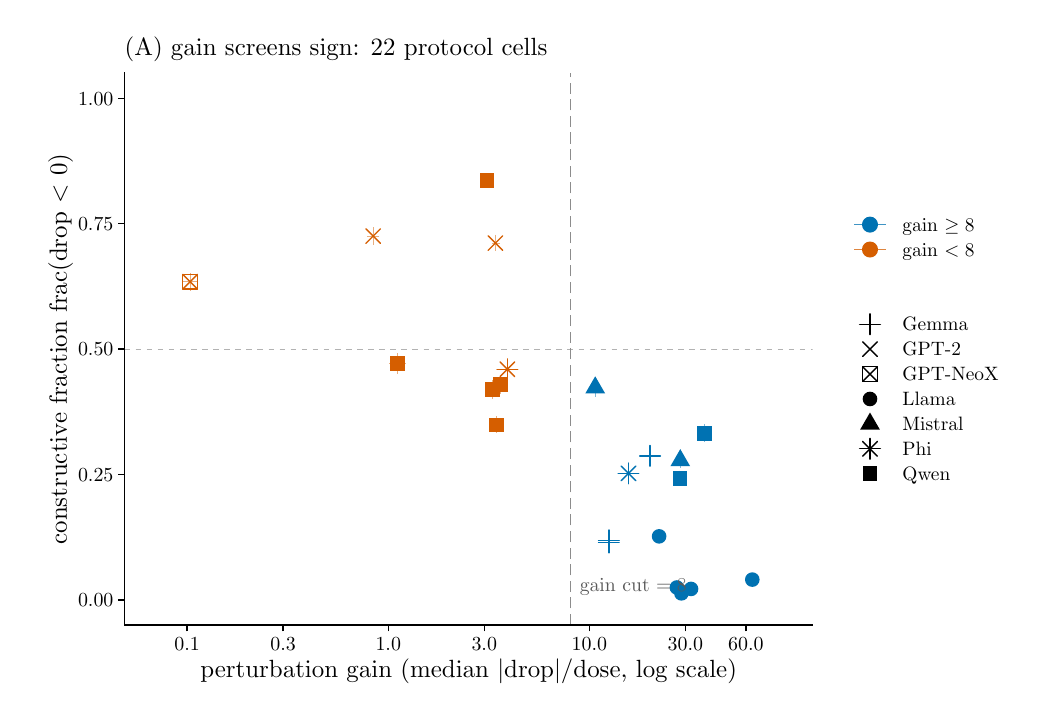
\begin{tikzpicture}[x=1pt,y=1pt]
\definecolor{fillColor}{RGB}{255,255,255}
\path[use as bounding box,fill=fillColor,fill opacity=0.00] (0,0) rectangle (361.35,238.49);
\begin{scope}
\path[clip] (  0.00,  0.00) rectangle (361.35,238.49);
\definecolor{drawColor}{RGB}{255,255,255}
\definecolor{fillColor}{RGB}{255,255,255}

\path[draw=drawColor,line width= 0.5pt,line join=round,line cap=round,fill=fillColor] (  0.00,  0.00) rectangle (361.35,238.49);
\end{scope}
\begin{scope}
\path[clip] ( 35.04, 22.61) rectangle (283.65,222.04);
\definecolor{fillColor}{RGB}{255,255,255}

\path[fill=fillColor] ( 35.04, 22.61) rectangle (283.65,222.04);
\definecolor{drawColor}{gray}{0.70}

\path[draw=drawColor,line width= 0.3pt,dash pattern=on 2pt off 2pt ,line join=round] ( 35.04,122.32) -- (283.65,122.32);
\definecolor{drawColor}{gray}{0.55}

\path[draw=drawColor,line width= 0.3pt,dash pattern=on 4pt off 2pt ,line join=round] (195.94, 22.61) -- (195.94,222.04);
\definecolor{drawColor}{RGB}{0,114,178}

\path[draw=drawColor,draw opacity=0.50,line width= 0.3pt,line join=round] (228.17, 56.80) --
	(228.17, 56.80);

\path[draw=drawColor,draw opacity=0.50,line width= 0.3pt,line join=round] (228.17, 56.80) --
	(228.17, 52.50);

\path[draw=drawColor,draw opacity=0.50,line width= 0.3pt,line join=round] (228.17, 52.50) --
	(228.17, 52.50);

\path[draw=drawColor,draw opacity=0.50,line width= 0.3pt,line join=round] (234.58, 37.30) --
	(234.58, 37.30);

\path[draw=drawColor,draw opacity=0.50,line width= 0.3pt,line join=round] (234.58, 37.30) --
	(234.58, 35.19);

\path[draw=drawColor,draw opacity=0.50,line width= 0.3pt,line join=round] (234.58, 35.19) --
	(234.58, 35.19);

\path[draw=drawColor,draw opacity=0.50,line width= 0.3pt,line join=round] (236.23, 34.85) --
	(236.23, 34.85);

\path[draw=drawColor,draw opacity=0.50,line width= 0.3pt,line join=round] (236.23, 34.85) --
	(236.23, 33.33);

\path[draw=drawColor,draw opacity=0.50,line width= 0.3pt,line join=round] (236.23, 33.33) --
	(236.23, 33.33);

\path[draw=drawColor,draw opacity=0.50,line width= 0.3pt,line join=round] (261.84, 40.40) --
	(261.84, 40.40);

\path[draw=drawColor,draw opacity=0.50,line width= 0.3pt,line join=round] (261.84, 40.40) --
	(261.84, 37.71);

\path[draw=drawColor,draw opacity=0.50,line width= 0.3pt,line join=round] (261.84, 37.71) --
	(261.84, 37.71);

\path[draw=drawColor,draw opacity=0.50,line width= 0.3pt,line join=round] (239.71, 36.70) --
	(239.71, 36.70);

\path[draw=drawColor,draw opacity=0.50,line width= 0.3pt,line join=round] (239.71, 36.70) --
	(239.71, 34.76);

\path[draw=drawColor,draw opacity=0.50,line width= 0.3pt,line join=round] (239.71, 34.76) --
	(239.71, 34.76);

\path[draw=drawColor,draw opacity=0.50,line width= 0.3pt,line join=round] (235.82, 84.92) --
	(235.82, 84.92);

\path[draw=drawColor,draw opacity=0.50,line width= 0.3pt,line join=round] (235.82, 84.92) --
	(235.82, 79.21);

\path[draw=drawColor,draw opacity=0.50,line width= 0.3pt,line join=round] (235.82, 79.21) --
	(235.82, 79.21);

\path[draw=drawColor,draw opacity=0.50,line width= 0.3pt,line join=round] (205.08,111.70) --
	(205.08,111.70);

\path[draw=drawColor,draw opacity=0.50,line width= 0.3pt,line join=round] (205.08,111.70) --
	(205.08,105.01);

\path[draw=drawColor,draw opacity=0.50,line width= 0.3pt,line join=round] (205.08,105.01) --
	(205.08,105.01);

\path[draw=drawColor,draw opacity=0.50,line width= 0.3pt,line join=round] (217.09, 80.38) --
	(217.09, 80.38);

\path[draw=drawColor,draw opacity=0.50,line width= 0.3pt,line join=round] (217.09, 80.38) --
	(217.09, 74.62);

\path[draw=drawColor,draw opacity=0.50,line width= 0.3pt,line join=round] (217.09, 74.62) --
	(217.09, 74.62);
\definecolor{drawColor}{RGB}{213,94,0}

\path[draw=drawColor,draw opacity=0.50,line width= 0.3pt,line join=round] (173.34,118.33) --
	(173.34,118.33);

\path[draw=drawColor,draw opacity=0.50,line width= 0.3pt,line join=round] (173.34,118.33) --
	(173.34,111.68);

\path[draw=drawColor,draw opacity=0.50,line width= 0.3pt,line join=round] (173.34,111.68) --
	(173.34,111.68);
\definecolor{drawColor}{RGB}{0,114,178}

\path[draw=drawColor,draw opacity=0.50,line width= 0.3pt,line join=round] (235.65, 78.43) --
	(235.65, 78.43);

\path[draw=drawColor,draw opacity=0.50,line width= 0.3pt,line join=round] (235.65, 78.43) --
	(235.65, 72.76);

\path[draw=drawColor,draw opacity=0.50,line width= 0.3pt,line join=round] (235.65, 72.76) --
	(235.65, 72.76);
\definecolor{drawColor}{RGB}{213,94,0}

\path[draw=drawColor,draw opacity=0.50,line width= 0.3pt,line join=round] (167.97,111.00) --
	(167.97,111.00);

\path[draw=drawColor,draw opacity=0.50,line width= 0.3pt,line join=round] (167.97,111.00) --
	(167.97,104.39);

\path[draw=drawColor,draw opacity=0.50,line width= 0.3pt,line join=round] (167.97,104.39) --
	(167.97,104.39);

\path[draw=drawColor,draw opacity=0.50,line width= 0.3pt,line join=round] (133.59,120.90) --
	(133.59,120.90);

\path[draw=drawColor,draw opacity=0.50,line width= 0.3pt,line join=round] (133.59,120.90) --
	(133.59,113.23);

\path[draw=drawColor,draw opacity=0.50,line width= 0.3pt,line join=round] (133.59,113.23) --
	(133.59,113.23);

\path[draw=drawColor,draw opacity=0.50,line width= 0.3pt,line join=round] (166.03,185.70) --
	(166.03,185.70);

\path[draw=drawColor,draw opacity=0.50,line width= 0.3pt,line join=round] (166.03,185.70) --
	(166.03,180.77);

\path[draw=drawColor,draw opacity=0.50,line width= 0.3pt,line join=round] (166.03,180.77) --
	(166.03,180.77);
\definecolor{drawColor}{RGB}{0,114,178}

\path[draw=drawColor,draw opacity=0.50,line width= 0.3pt,line join=round] (244.49, 95.19) --
	(244.49, 95.19);

\path[draw=drawColor,draw opacity=0.50,line width= 0.3pt,line join=round] (244.49, 95.19) --
	(244.49, 88.62);

\path[draw=drawColor,draw opacity=0.50,line width= 0.3pt,line join=round] (244.49, 88.62) --
	(244.49, 88.62);
\definecolor{drawColor}{RGB}{213,94,0}

\path[draw=drawColor,draw opacity=0.50,line width= 0.3pt,line join=round] (170.95,112.73) --
	(170.95,112.73);

\path[draw=drawColor,draw opacity=0.50,line width= 0.3pt,line join=round] (170.95,112.73) --
	(170.95,106.29);

\path[draw=drawColor,draw opacity=0.50,line width= 0.3pt,line join=round] (170.95,106.29) --
	(170.95,106.29);

\path[draw=drawColor,draw opacity=0.50,line width= 0.3pt,line join=round] (169.40, 98.12) --
	(169.40, 98.12);

\path[draw=drawColor,draw opacity=0.50,line width= 0.3pt,line join=round] (169.40, 98.12) --
	(169.40, 91.94);

\path[draw=drawColor,draw opacity=0.50,line width= 0.3pt,line join=round] (169.40, 91.94) --
	(169.40, 91.94);
\definecolor{drawColor}{RGB}{0,114,178}

\path[draw=drawColor,draw opacity=0.50,line width= 0.3pt,line join=round] (224.89, 86.86) --
	(224.89, 86.86);

\path[draw=drawColor,draw opacity=0.50,line width= 0.3pt,line join=round] (224.89, 86.86) --
	(224.89, 80.70);

\path[draw=drawColor,draw opacity=0.50,line width= 0.3pt,line join=round] (224.89, 80.70) --
	(224.89, 80.70);

\path[draw=drawColor,draw opacity=0.50,line width= 0.3pt,line join=round] (209.99, 54.53) --
	(209.99, 54.53);

\path[draw=drawColor,draw opacity=0.50,line width= 0.3pt,line join=round] (209.99, 54.53) --
	(209.99, 50.34);

\path[draw=drawColor,draw opacity=0.50,line width= 0.3pt,line join=round] (209.99, 50.34) --
	(209.99, 50.34);

\path[draw=drawColor,draw opacity=0.50,line width= 0.3pt,line join=round] (210.01, 55.44) --
	(210.01, 55.44);

\path[draw=drawColor,draw opacity=0.50,line width= 0.3pt,line join=round] (210.01, 55.44) --
	(210.01, 51.18);

\path[draw=drawColor,draw opacity=0.50,line width= 0.3pt,line join=round] (210.01, 51.18) --
	(210.01, 51.18);
\definecolor{drawColor}{RGB}{213,94,0}

\path[draw=drawColor,draw opacity=0.50,line width= 0.3pt,line join=round] ( 58.69,149.92) --
	( 58.69,149.92);

\path[draw=drawColor,draw opacity=0.50,line width= 0.3pt,line join=round] ( 58.69,149.92) --
	( 58.69,143.38);

\path[draw=drawColor,draw opacity=0.50,line width= 0.3pt,line join=round] ( 58.69,143.38) --
	( 58.69,143.38);

\path[draw=drawColor,draw opacity=0.50,line width= 0.3pt,line join=round] (169.02,163.68) --
	(169.02,163.68);

\path[draw=drawColor,draw opacity=0.50,line width= 0.3pt,line join=round] (169.02,163.68) --
	(169.02,157.64);

\path[draw=drawColor,draw opacity=0.50,line width= 0.3pt,line join=round] (169.02,157.64) --
	(169.02,157.64);

\path[draw=drawColor,draw opacity=0.50,line width= 0.3pt,line join=round] (124.84,166.36) --
	(124.84,166.36);

\path[draw=drawColor,draw opacity=0.50,line width= 0.3pt,line join=round] (124.84,166.36) --
	(124.84,159.82);

\path[draw=drawColor,draw opacity=0.50,line width= 0.3pt,line join=round] (124.84,159.82) --
	(124.84,159.82);
\definecolor{drawColor}{RGB}{0,114,178}

\path[draw=drawColor,draw opacity=0.50,line width= 0.3pt,line join=round] (229.30, 54.68) --
	(229.30, 54.68);

\path[draw=drawColor,draw opacity=0.50,line width= 0.3pt,line join=round] (229.30, 54.68) --
	(227.10, 54.68);

\path[draw=drawColor,draw opacity=0.50,line width= 0.3pt,line join=round] (227.10, 54.68) --
	(227.10, 54.68);

\path[draw=drawColor,draw opacity=0.50,line width= 0.3pt,line join=round] (235.72, 36.20) --
	(235.72, 36.20);

\path[draw=drawColor,draw opacity=0.50,line width= 0.3pt,line join=round] (235.72, 36.20) --
	(233.36, 36.20);

\path[draw=drawColor,draw opacity=0.50,line width= 0.3pt,line join=round] (233.36, 36.20) --
	(233.36, 36.20);

\path[draw=drawColor,draw opacity=0.50,line width= 0.3pt,line join=round] (237.41, 34.08) --
	(237.41, 34.08);

\path[draw=drawColor,draw opacity=0.50,line width= 0.3pt,line join=round] (237.41, 34.08) --
	(234.86, 34.08);

\path[draw=drawColor,draw opacity=0.50,line width= 0.3pt,line join=round] (234.86, 34.08) --
	(234.86, 34.08);

\path[draw=drawColor,draw opacity=0.50,line width= 0.3pt,line join=round] (263.33, 39.05) --
	(263.33, 39.05);

\path[draw=drawColor,draw opacity=0.50,line width= 0.3pt,line join=round] (263.33, 39.05) --
	(260.55, 39.05);

\path[draw=drawColor,draw opacity=0.50,line width= 0.3pt,line join=round] (260.55, 39.05) --
	(260.55, 39.05);

\path[draw=drawColor,draw opacity=0.50,line width= 0.3pt,line join=round] (240.62, 35.68) --
	(240.62, 35.68);

\path[draw=drawColor,draw opacity=0.50,line width= 0.3pt,line join=round] (240.62, 35.68) --
	(238.95, 35.68);

\path[draw=drawColor,draw opacity=0.50,line width= 0.3pt,line join=round] (238.95, 35.68) --
	(238.95, 35.68);

\path[draw=drawColor,draw opacity=0.50,line width= 0.3pt,line join=round] (237.62, 82.09) --
	(237.62, 82.09);

\path[draw=drawColor,draw opacity=0.50,line width= 0.3pt,line join=round] (237.62, 82.09) --
	(234.63, 82.09);

\path[draw=drawColor,draw opacity=0.50,line width= 0.3pt,line join=round] (234.63, 82.09) --
	(234.63, 82.09);

\path[draw=drawColor,draw opacity=0.50,line width= 0.3pt,line join=round] (206.58,108.42) --
	(206.58,108.42);

\path[draw=drawColor,draw opacity=0.50,line width= 0.3pt,line join=round] (206.58,108.42) --
	(203.69,108.42);

\path[draw=drawColor,draw opacity=0.50,line width= 0.3pt,line join=round] (203.69,108.42) --
	(203.69,108.42);

\path[draw=drawColor,draw opacity=0.50,line width= 0.3pt,line join=round] (218.47, 77.43) --
	(218.47, 77.43);

\path[draw=drawColor,draw opacity=0.50,line width= 0.3pt,line join=round] (218.47, 77.43) --
	(215.54, 77.43);

\path[draw=drawColor,draw opacity=0.50,line width= 0.3pt,line join=round] (215.54, 77.43) --
	(215.54, 77.43);
\definecolor{drawColor}{RGB}{213,94,0}

\path[draw=drawColor,draw opacity=0.50,line width= 0.3pt,line join=round] (175.16,115.07) --
	(175.16,115.07);

\path[draw=drawColor,draw opacity=0.50,line width= 0.3pt,line join=round] (175.16,115.07) --
	(171.74,115.07);

\path[draw=drawColor,draw opacity=0.50,line width= 0.3pt,line join=round] (171.74,115.07) --
	(171.74,115.07);
\definecolor{drawColor}{RGB}{0,114,178}

\path[draw=drawColor,draw opacity=0.50,line width= 0.3pt,line join=round] (237.25, 75.62) --
	(237.25, 75.62);

\path[draw=drawColor,draw opacity=0.50,line width= 0.3pt,line join=round] (237.25, 75.62) --
	(234.14, 75.62);

\path[draw=drawColor,draw opacity=0.50,line width= 0.3pt,line join=round] (234.14, 75.62) --
	(234.14, 75.62);
\definecolor{drawColor}{RGB}{213,94,0}

\path[draw=drawColor,draw opacity=0.50,line width= 0.3pt,line join=round] (169.51,107.77) --
	(169.51,107.77);

\path[draw=drawColor,draw opacity=0.50,line width= 0.3pt,line join=round] (169.51,107.77) --
	(165.80,107.77);

\path[draw=drawColor,draw opacity=0.50,line width= 0.3pt,line join=round] (165.80,107.77) --
	(165.80,107.77);

\path[draw=drawColor,draw opacity=0.50,line width= 0.3pt,line join=round] (136.60,117.07) --
	(136.60,117.07);

\path[draw=drawColor,draw opacity=0.50,line width= 0.3pt,line join=round] (136.60,117.07) --
	(130.66,117.07);

\path[draw=drawColor,draw opacity=0.50,line width= 0.3pt,line join=round] (130.66,117.07) --
	(130.66,117.07);

\path[draw=drawColor,draw opacity=0.50,line width= 0.3pt,line join=round] (167.49,183.30) --
	(167.49,183.30);

\path[draw=drawColor,draw opacity=0.50,line width= 0.3pt,line join=round] (167.49,183.30) --
	(164.44,183.30);

\path[draw=drawColor,draw opacity=0.50,line width= 0.3pt,line join=round] (164.44,183.30) --
	(164.44,183.30);
\definecolor{drawColor}{RGB}{0,114,178}

\path[draw=drawColor,draw opacity=0.50,line width= 0.3pt,line join=round] (246.28, 91.94) --
	(246.28, 91.94);

\path[draw=drawColor,draw opacity=0.50,line width= 0.3pt,line join=round] (246.28, 91.94) --
	(242.51, 91.94);

\path[draw=drawColor,draw opacity=0.50,line width= 0.3pt,line join=round] (242.51, 91.94) --
	(242.51, 91.94);
\definecolor{drawColor}{RGB}{213,94,0}

\path[draw=drawColor,draw opacity=0.50,line width= 0.3pt,line join=round] (172.48,109.60) --
	(172.48,109.60);

\path[draw=drawColor,draw opacity=0.50,line width= 0.3pt,line join=round] (172.48,109.60) --
	(169.73,109.60);

\path[draw=drawColor,draw opacity=0.50,line width= 0.3pt,line join=round] (169.73,109.60) --
	(169.73,109.60);

\path[draw=drawColor,draw opacity=0.50,line width= 0.3pt,line join=round] (171.02, 94.91) --
	(171.02, 94.91);

\path[draw=drawColor,draw opacity=0.50,line width= 0.3pt,line join=round] (171.02, 94.91) --
	(167.61, 94.91);

\path[draw=drawColor,draw opacity=0.50,line width= 0.3pt,line join=round] (167.61, 94.91) --
	(167.61, 94.91);
\definecolor{drawColor}{RGB}{0,114,178}

\path[draw=drawColor,draw opacity=0.50,line width= 0.3pt,line join=round] (226.53, 83.78) --
	(226.53, 83.78);

\path[draw=drawColor,draw opacity=0.50,line width= 0.3pt,line join=round] (226.53, 83.78) --
	(223.04, 83.78);

\path[draw=drawColor,draw opacity=0.50,line width= 0.3pt,line join=round] (223.04, 83.78) --
	(223.04, 83.78);

\path[draw=drawColor,draw opacity=0.50,line width= 0.3pt,line join=round] (211.38, 52.47) --
	(211.38, 52.47);

\path[draw=drawColor,draw opacity=0.50,line width= 0.3pt,line join=round] (211.38, 52.47) --
	(208.34, 52.47);

\path[draw=drawColor,draw opacity=0.50,line width= 0.3pt,line join=round] (208.34, 52.47) --
	(208.34, 52.47);

\path[draw=drawColor,draw opacity=0.50,line width= 0.3pt,line join=round] (211.36, 53.25) --
	(211.36, 53.25);

\path[draw=drawColor,draw opacity=0.50,line width= 0.3pt,line join=round] (211.36, 53.25) --
	(208.48, 53.25);

\path[draw=drawColor,draw opacity=0.50,line width= 0.3pt,line join=round] (208.48, 53.25) --
	(208.48, 53.25);
\definecolor{drawColor}{RGB}{213,94,0}

\path[draw=drawColor,draw opacity=0.50,line width= 0.3pt,line join=round] ( 61.08,146.69) --
	( 61.08,146.69);

\path[draw=drawColor,draw opacity=0.50,line width= 0.3pt,line join=round] ( 61.08,146.69) --
	( 56.27,146.69);

\path[draw=drawColor,draw opacity=0.50,line width= 0.3pt,line join=round] ( 56.27,146.69) --
	( 56.27,146.69);

\path[draw=drawColor,draw opacity=0.50,line width= 0.3pt,line join=round] (170.59,160.65) --
	(170.59,160.65);

\path[draw=drawColor,draw opacity=0.50,line width= 0.3pt,line join=round] (170.59,160.65) --
	(167.64,160.65);

\path[draw=drawColor,draw opacity=0.50,line width= 0.3pt,line join=round] (167.64,160.65) --
	(167.64,160.65);

\path[draw=drawColor,draw opacity=0.50,line width= 0.3pt,line join=round] (127.05,163.17) --
	(127.05,163.17);

\path[draw=drawColor,draw opacity=0.50,line width= 0.3pt,line join=round] (127.05,163.17) --
	(122.48,163.17);

\path[draw=drawColor,draw opacity=0.50,line width= 0.3pt,line join=round] (122.48,163.17) --
	(122.48,163.17);
\definecolor{fillColor}{RGB}{0,114,178}

\path[fill=fillColor] (228.17, 54.68) circle (  2.64);

\path[fill=fillColor] (234.58, 36.20) circle (  2.64);

\path[fill=fillColor] (236.23, 34.08) circle (  2.64);

\path[fill=fillColor] (261.84, 39.05) circle (  2.64);

\path[fill=fillColor] (239.71, 35.68) circle (  2.64);

\path[fill=fillColor] (235.82, 86.20) --
	(239.37, 80.04) --
	(232.26, 80.04) --
	cycle;

\path[fill=fillColor] (205.08,112.52) --
	(208.64,106.37) --
	(201.53,106.37) --
	cycle;
\definecolor{drawColor}{RGB}{0,114,178}

\path[draw=drawColor,line width= 0.5pt,line join=round,line cap=round] (214.45, 74.79) -- (219.73, 80.07);

\path[draw=drawColor,line width= 0.5pt,line join=round,line cap=round] (214.45, 80.07) -- (219.73, 74.79);

\path[draw=drawColor,line width= 0.5pt,line join=round,line cap=round] (213.36, 77.43) -- (220.83, 77.43);

\path[draw=drawColor,line width= 0.5pt,line join=round,line cap=round] (217.09, 73.70) -- (217.09, 81.17);
\definecolor{drawColor}{RGB}{213,94,0}

\path[draw=drawColor,line width= 0.5pt,line join=round,line cap=round] (170.70,112.43) -- (175.98,117.71);

\path[draw=drawColor,line width= 0.5pt,line join=round,line cap=round] (170.70,117.71) -- (175.98,112.43);

\path[draw=drawColor,line width= 0.5pt,line join=round,line cap=round] (169.61,115.07) -- (177.07,115.07);

\path[draw=drawColor,line width= 0.5pt,line join=round,line cap=round] (173.34,111.34) -- (173.34,118.81);

\path[fill=fillColor] (233.02, 72.98) --
	(238.29, 72.98) --
	(238.29, 78.26) --
	(233.02, 78.26) --
	cycle;
\definecolor{fillColor}{RGB}{213,94,0}

\path[fill=fillColor] (165.33,105.13) --
	(170.61,105.13) --
	(170.61,110.41) --
	(165.33,110.41) --
	cycle;

\path[fill=fillColor] (130.95,114.43) --
	(136.23,114.43) --
	(136.23,119.71) --
	(130.95,119.71) --
	cycle;

\path[fill=fillColor] (163.39,180.66) --
	(168.67,180.66) --
	(168.67,185.94) --
	(163.39,185.94) --
	cycle;
\definecolor{fillColor}{RGB}{0,114,178}

\path[fill=fillColor] (241.85, 89.30) --
	(247.13, 89.30) --
	(247.13, 94.58) --
	(241.85, 94.58) --
	cycle;
\definecolor{fillColor}{RGB}{213,94,0}

\path[fill=fillColor] (168.31,106.96) --
	(173.59,106.96) --
	(173.59,112.24) --
	(168.31,112.24) --
	cycle;

\path[fill=fillColor] (166.76, 92.27) --
	(172.04, 92.27) --
	(172.04, 97.55) --
	(166.76, 97.55) --
	cycle;
\definecolor{drawColor}{RGB}{0,114,178}

\path[draw=drawColor,line width= 0.5pt,line join=round,line cap=round] (221.16, 83.78) -- (228.63, 83.78);

\path[draw=drawColor,line width= 0.5pt,line join=round,line cap=round] (224.89, 80.05) -- (224.89, 87.51);

\path[draw=drawColor,line width= 0.5pt,line join=round,line cap=round] (206.25, 52.47) -- (213.72, 52.47);

\path[draw=drawColor,line width= 0.5pt,line join=round,line cap=round] (209.99, 48.73) -- (209.99, 56.20);

\path[draw=drawColor,line width= 0.5pt,line join=round,line cap=round] (206.27, 53.25) -- (213.74, 53.25);

\path[draw=drawColor,line width= 0.5pt,line join=round,line cap=round] (210.01, 49.51) -- (210.01, 56.98);
\definecolor{drawColor}{RGB}{213,94,0}

\path[draw=drawColor,line width= 0.5pt,line join=round,line cap=round] ( 56.05,144.05) rectangle ( 61.33,149.33);

\path[draw=drawColor,line width= 0.5pt,line join=round,line cap=round] ( 56.05,144.05) -- ( 61.33,149.33);

\path[draw=drawColor,line width= 0.5pt,line join=round,line cap=round] ( 56.05,149.33) -- ( 61.33,144.05);

\path[draw=drawColor,line width= 0.5pt,line join=round,line cap=round] (166.38,158.01) -- (171.66,163.29);

\path[draw=drawColor,line width= 0.5pt,line join=round,line cap=round] (166.38,163.29) -- (171.66,158.01);

\path[draw=drawColor,line width= 0.5pt,line join=round,line cap=round] (122.20,160.53) -- (127.48,165.81);

\path[draw=drawColor,line width= 0.5pt,line join=round,line cap=round] (122.20,165.81) -- (127.48,160.53);
\definecolor{drawColor}{gray}{0.35}

\node[text=drawColor,anchor=base west,inner sep=0pt, outer sep=0pt, scale=  0.71] at (199.52, 34.66) {gain cut $=8$};
\end{scope}
\begin{scope}
\path[clip] (  0.00,  0.00) rectangle (361.35,238.49);
\definecolor{drawColor}{RGB}{0,0,0}

\path[draw=drawColor,line width= 0.5pt,line join=round,line cap=rect] ( 35.04, 22.61) --
	( 35.04,222.04);
\end{scope}
\begin{scope}
\path[clip] (  0.00,  0.00) rectangle (361.35,238.49);
\definecolor{drawColor}{RGB}{0,0,0}

\node[text=drawColor,anchor=base east,inner sep=0pt, outer sep=0pt, scale=  0.72] at ( 30.99, 29.19) {0.00};

\node[text=drawColor,anchor=base east,inner sep=0pt, outer sep=0pt, scale=  0.72] at ( 30.99, 74.52) {0.25};

\node[text=drawColor,anchor=base east,inner sep=0pt, outer sep=0pt, scale=  0.72] at ( 30.99,119.85) {0.50};

\node[text=drawColor,anchor=base east,inner sep=0pt, outer sep=0pt, scale=  0.72] at ( 30.99,165.17) {0.75};

\node[text=drawColor,anchor=base east,inner sep=0pt, outer sep=0pt, scale=  0.72] at ( 30.99,210.50) {1.00};
\end{scope}
\begin{scope}
\path[clip] (  0.00,  0.00) rectangle (361.35,238.49);
\definecolor{drawColor}{RGB}{0,0,0}

\path[draw=drawColor,line width= 0.5pt,line join=round] ( 32.79, 31.67) --
	( 35.04, 31.67);

\path[draw=drawColor,line width= 0.5pt,line join=round] ( 32.79, 77.00) --
	( 35.04, 77.00);

\path[draw=drawColor,line width= 0.5pt,line join=round] ( 32.79,122.32) --
	( 35.04,122.32);

\path[draw=drawColor,line width= 0.5pt,line join=round] ( 32.79,167.65) --
	( 35.04,167.65);

\path[draw=drawColor,line width= 0.5pt,line join=round] ( 32.79,212.98) --
	( 35.04,212.98);
\end{scope}
\begin{scope}
\path[clip] (  0.00,  0.00) rectangle (361.35,238.49);
\definecolor{drawColor}{RGB}{0,0,0}

\path[draw=drawColor,line width= 0.5pt,line join=round,line cap=rect] ( 35.04, 22.61) --
	(283.65, 22.61);
\end{scope}
\begin{scope}
\path[clip] (  0.00,  0.00) rectangle (361.35,238.49);
\definecolor{drawColor}{RGB}{0,0,0}

\path[draw=drawColor,line width= 0.5pt,line join=round] ( 57.60, 20.36) --
	( 57.60, 22.61);

\path[draw=drawColor,line width= 0.5pt,line join=round] ( 92.29, 20.36) --
	( 92.29, 22.61);

\path[draw=drawColor,line width= 0.5pt,line join=round] (130.29, 20.36) --
	(130.29, 22.61);

\path[draw=drawColor,line width= 0.5pt,line join=round] (164.98, 20.36) --
	(164.98, 22.61);

\path[draw=drawColor,line width= 0.5pt,line join=round] (202.98, 20.36) --
	(202.98, 22.61);

\path[draw=drawColor,line width= 0.5pt,line join=round] (237.67, 20.36) --
	(237.67, 22.61);

\path[draw=drawColor,line width= 0.5pt,line join=round] (259.55, 20.36) --
	(259.55, 22.61);
\end{scope}
\begin{scope}
\path[clip] (  0.00,  0.00) rectangle (361.35,238.49);
\definecolor{drawColor}{RGB}{0,0,0}

\node[text=drawColor,anchor=base,inner sep=0pt, outer sep=0pt, scale=  0.72] at ( 57.60, 13.60) {0.1};

\node[text=drawColor,anchor=base,inner sep=0pt, outer sep=0pt, scale=  0.72] at ( 92.29, 13.60) {0.3};

\node[text=drawColor,anchor=base,inner sep=0pt, outer sep=0pt, scale=  0.72] at (130.29, 13.60) {1.0};

\node[text=drawColor,anchor=base,inner sep=0pt, outer sep=0pt, scale=  0.72] at (164.98, 13.60) {3.0};

\node[text=drawColor,anchor=base,inner sep=0pt, outer sep=0pt, scale=  0.72] at (202.98, 13.60) {10.0};

\node[text=drawColor,anchor=base,inner sep=0pt, outer sep=0pt, scale=  0.72] at (237.67, 13.60) {30.0};

\node[text=drawColor,anchor=base,inner sep=0pt, outer sep=0pt, scale=  0.72] at (259.55, 13.60) {60.0};
\end{scope}
\begin{scope}
\path[clip] (  0.00,  0.00) rectangle (361.35,238.49);
\definecolor{drawColor}{RGB}{0,0,0}

\node[text=drawColor,anchor=base,inner sep=0pt, outer sep=0pt, scale=  0.90] at (159.35,  3.75) {perturbation gain (median $|$drop$|$/dose, log scale)};
\end{scope}
\begin{scope}
\path[clip] (  0.00,  0.00) rectangle (361.35,238.49);
\definecolor{drawColor}{RGB}{0,0,0}

\node[text=drawColor,rotate= 90.00,anchor=base,inner sep=0pt, outer sep=0pt, scale=  0.90] at ( 14.20,122.32) {constructive fraction  frac(drop $<$ 0)};
\end{scope}
\begin{scope}
\path[clip] (  0.00,  0.00) rectangle (361.35,238.49);
\definecolor{fillColor}{RGB}{255,255,255}

\path[fill=fillColor] (292.65,149.32) rectangle (346.65,176.32);
\end{scope}
\begin{scope}
\path[clip] (  0.00,  0.00) rectangle (361.35,238.49);
\definecolor{fillColor}{RGB}{255,255,255}

\path[fill=fillColor] (297.15,162.82) rectangle (311.60,171.82);
\definecolor{drawColor}{RGB}{0,114,178}

\path[draw=drawColor,draw opacity=0.50,line width= 0.3pt,line join=round] (298.59,167.32) -- (310.16,167.32);

\path[draw=drawColor,draw opacity=0.50,line width= 0.3pt,line join=round] (298.59,167.32) -- (310.16,167.32);
\definecolor{drawColor}{RGB}{0,114,178}
\definecolor{fillColor}{RGB}{0,114,178}

\path[draw=drawColor,line width= 0.5pt,line join=round,line cap=round,fill=fillColor] (304.37,167.32) circle (  2.64);
\end{scope}
\begin{scope}
\path[clip] (  0.00,  0.00) rectangle (361.35,238.49);
\definecolor{fillColor}{RGB}{255,255,255}

\path[fill=fillColor] (297.15,153.82) rectangle (311.60,162.82);
\definecolor{drawColor}{RGB}{213,94,0}

\path[draw=drawColor,draw opacity=0.50,line width= 0.3pt,line join=round] (298.59,158.32) -- (310.16,158.32);

\path[draw=drawColor,draw opacity=0.50,line width= 0.3pt,line join=round] (298.59,158.32) -- (310.16,158.32);
\definecolor{drawColor}{RGB}{213,94,0}
\definecolor{fillColor}{RGB}{213,94,0}

\path[draw=drawColor,line width= 0.5pt,line join=round,line cap=round,fill=fillColor] (304.37,158.32) circle (  2.64);
\end{scope}
\begin{scope}
\path[clip] (  0.00,  0.00) rectangle (361.35,238.49);
\definecolor{drawColor}{RGB}{0,0,0}

\node[text=drawColor,anchor=base west,inner sep=0pt, outer sep=0pt, scale=  0.70] at (316.10,164.91) {gain $\geq 8$};
\end{scope}
\begin{scope}
\path[clip] (  0.00,  0.00) rectangle (361.35,238.49);
\definecolor{drawColor}{RGB}{0,0,0}

\node[text=drawColor,anchor=base west,inner sep=0pt, outer sep=0pt, scale=  0.70] at (316.10,155.91) {gain $< 8$};
\end{scope}
\begin{scope}
\path[clip] (  0.00,  0.00) rectangle (361.35,238.49);
\definecolor{fillColor}{RGB}{255,255,255}

\path[fill=fillColor] (292.65, 68.32) rectangle (355.35,140.32);
\end{scope}
\begin{scope}
\path[clip] (  0.00,  0.00) rectangle (361.35,238.49);
\definecolor{fillColor}{RGB}{255,255,255}

\path[fill=fillColor] (297.15,126.82) rectangle (311.60,135.82);
\definecolor{drawColor}{RGB}{0,0,0}

\path[draw=drawColor,line width= 0.5pt,line join=round,line cap=round] (300.64,131.32) -- (308.11,131.32);

\path[draw=drawColor,line width= 0.5pt,line join=round,line cap=round] (304.37,127.59) -- (304.37,135.06);
\end{scope}
\begin{scope}
\path[clip] (  0.00,  0.00) rectangle (361.35,238.49);
\definecolor{fillColor}{RGB}{255,255,255}

\path[fill=fillColor] (297.15,117.82) rectangle (311.60,126.82);
\definecolor{drawColor}{RGB}{0,0,0}

\path[draw=drawColor,line width= 0.5pt,line join=round,line cap=round] (301.73,119.68) -- (307.01,124.96);

\path[draw=drawColor,line width= 0.5pt,line join=round,line cap=round] (301.73,124.96) -- (307.01,119.68);
\end{scope}
\begin{scope}
\path[clip] (  0.00,  0.00) rectangle (361.35,238.49);
\definecolor{fillColor}{RGB}{255,255,255}

\path[fill=fillColor] (297.15,108.82) rectangle (311.60,117.82);
\definecolor{drawColor}{RGB}{0,0,0}

\path[draw=drawColor,line width= 0.5pt,line join=round,line cap=round] (301.73,110.68) rectangle (307.01,115.96);

\path[draw=drawColor,line width= 0.5pt,line join=round,line cap=round] (301.73,110.68) -- (307.01,115.96);

\path[draw=drawColor,line width= 0.5pt,line join=round,line cap=round] (301.73,115.96) -- (307.01,110.68);
\end{scope}
\begin{scope}
\path[clip] (  0.00,  0.00) rectangle (361.35,238.49);
\definecolor{fillColor}{RGB}{255,255,255}

\path[fill=fillColor] (297.15, 99.82) rectangle (311.60,108.82);
\definecolor{fillColor}{RGB}{0,0,0}

\path[fill=fillColor] (304.37,104.32) circle (  2.64);
\end{scope}
\begin{scope}
\path[clip] (  0.00,  0.00) rectangle (361.35,238.49);
\definecolor{fillColor}{RGB}{255,255,255}

\path[fill=fillColor] (297.15, 90.82) rectangle (311.60, 99.82);
\definecolor{fillColor}{RGB}{0,0,0}

\path[fill=fillColor] (304.37, 99.43) --
	(307.93, 93.27) --
	(300.82, 93.27) --
	cycle;
\end{scope}
\begin{scope}
\path[clip] (  0.00,  0.00) rectangle (361.35,238.49);
\definecolor{fillColor}{RGB}{255,255,255}

\path[fill=fillColor] (297.15, 81.82) rectangle (311.60, 90.82);
\definecolor{drawColor}{RGB}{0,0,0}

\path[draw=drawColor,line width= 0.5pt,line join=round,line cap=round] (301.73, 83.68) -- (307.01, 88.96);

\path[draw=drawColor,line width= 0.5pt,line join=round,line cap=round] (301.73, 88.96) -- (307.01, 83.68);

\path[draw=drawColor,line width= 0.5pt,line join=round,line cap=round] (300.64, 86.32) -- (308.11, 86.32);

\path[draw=drawColor,line width= 0.5pt,line join=round,line cap=round] (304.37, 82.59) -- (304.37, 90.06);
\end{scope}
\begin{scope}
\path[clip] (  0.00,  0.00) rectangle (361.35,238.49);
\definecolor{fillColor}{RGB}{255,255,255}

\path[fill=fillColor] (297.15, 72.82) rectangle (311.60, 81.82);
\definecolor{fillColor}{RGB}{0,0,0}

\path[fill=fillColor] (301.73, 74.68) --
	(307.01, 74.68) --
	(307.01, 79.96) --
	(301.73, 79.96) --
	cycle;
\end{scope}
\begin{scope}
\path[clip] (  0.00,  0.00) rectangle (361.35,238.49);
\definecolor{drawColor}{RGB}{0,0,0}

\node[text=drawColor,anchor=base west,inner sep=0pt, outer sep=0pt, scale=  0.70] at (316.10,128.91) {Gemma};
\end{scope}
\begin{scope}
\path[clip] (  0.00,  0.00) rectangle (361.35,238.49);
\definecolor{drawColor}{RGB}{0,0,0}

\node[text=drawColor,anchor=base west,inner sep=0pt, outer sep=0pt, scale=  0.70] at (316.10,119.91) {GPT-2};
\end{scope}
\begin{scope}
\path[clip] (  0.00,  0.00) rectangle (361.35,238.49);
\definecolor{drawColor}{RGB}{0,0,0}

\node[text=drawColor,anchor=base west,inner sep=0pt, outer sep=0pt, scale=  0.70] at (316.10,110.91) {GPT-NeoX};
\end{scope}
\begin{scope}
\path[clip] (  0.00,  0.00) rectangle (361.35,238.49);
\definecolor{drawColor}{RGB}{0,0,0}

\node[text=drawColor,anchor=base west,inner sep=0pt, outer sep=0pt, scale=  0.70] at (316.10,101.91) {Llama};
\end{scope}
\begin{scope}
\path[clip] (  0.00,  0.00) rectangle (361.35,238.49);
\definecolor{drawColor}{RGB}{0,0,0}

\node[text=drawColor,anchor=base west,inner sep=0pt, outer sep=0pt, scale=  0.70] at (316.10, 92.91) {Mistral};
\end{scope}
\begin{scope}
\path[clip] (  0.00,  0.00) rectangle (361.35,238.49);
\definecolor{drawColor}{RGB}{0,0,0}

\node[text=drawColor,anchor=base west,inner sep=0pt, outer sep=0pt, scale=  0.70] at (316.10, 83.91) {Phi};
\end{scope}
\begin{scope}
\path[clip] (  0.00,  0.00) rectangle (361.35,238.49);
\definecolor{drawColor}{RGB}{0,0,0}

\node[text=drawColor,anchor=base west,inner sep=0pt, outer sep=0pt, scale=  0.70] at (316.10, 74.91) {Qwen};
\end{scope}
\begin{scope}
\path[clip] (  0.00,  0.00) rectangle (361.35,238.49);
\definecolor{drawColor}{RGB}{0,0,0}

\node[text=drawColor,anchor=base west,inner sep=0pt, outer sep=0pt, scale=  0.90] at ( 35.04,228.29) {(A) gain screens sign: 22 protocol cells};
\end{scope}
\end{tikzpicture}
